\section{Optimization Studies}

\subsection{Combined Mass impact}
\label{sec:app-optimization-cbmass}
\paragraph{}
Using combined mass instead of the calorimeter based mass improves the boosted exclusion limit across the mass range, as can be seen in ~\ref{fig:app-optimization-mass}.

\begin{figure*}[htbp!]
\begin{center}
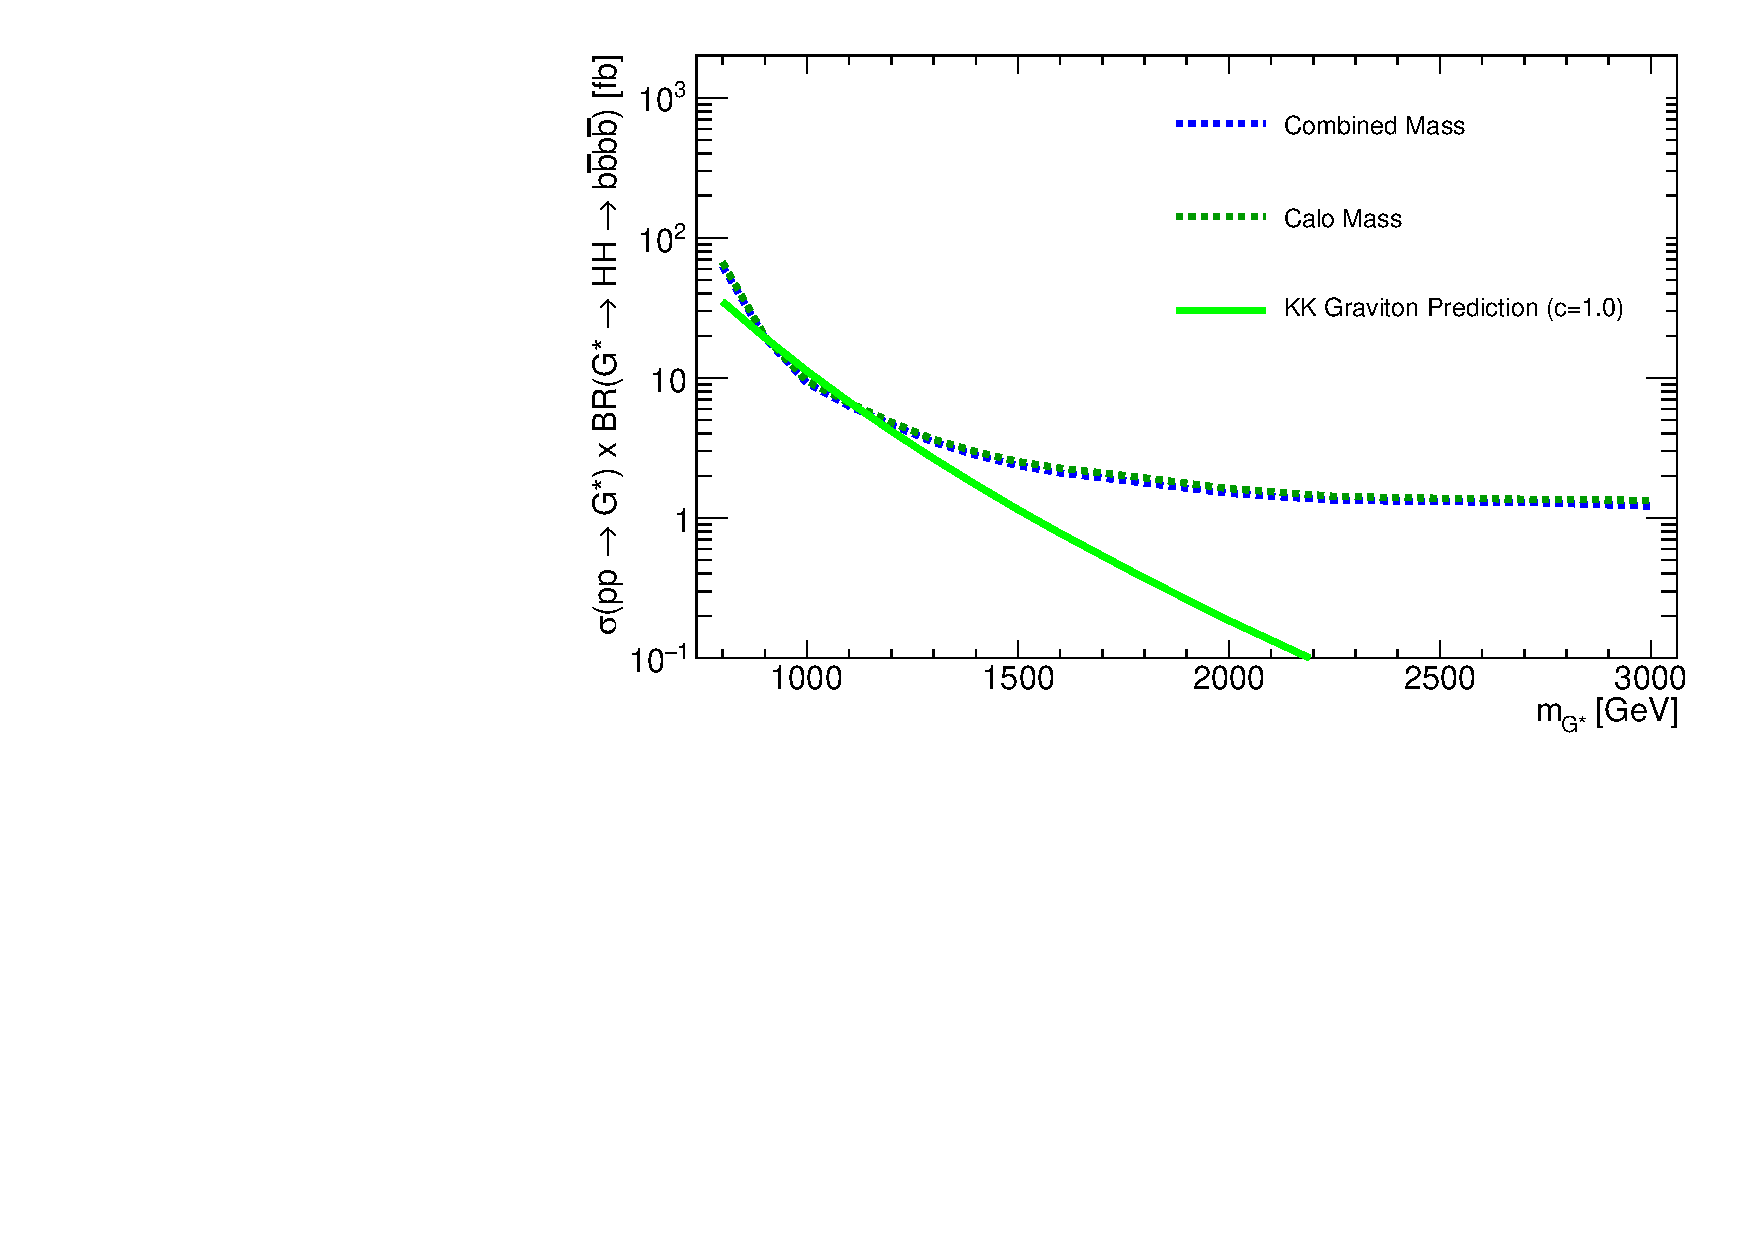
\includegraphics[angle=270, width=0.68\textwidth]{./figures/boosted/AppendixOptimization/CompareLimits_HH_BoostedNewRun2-mass_c10.pdf}\\
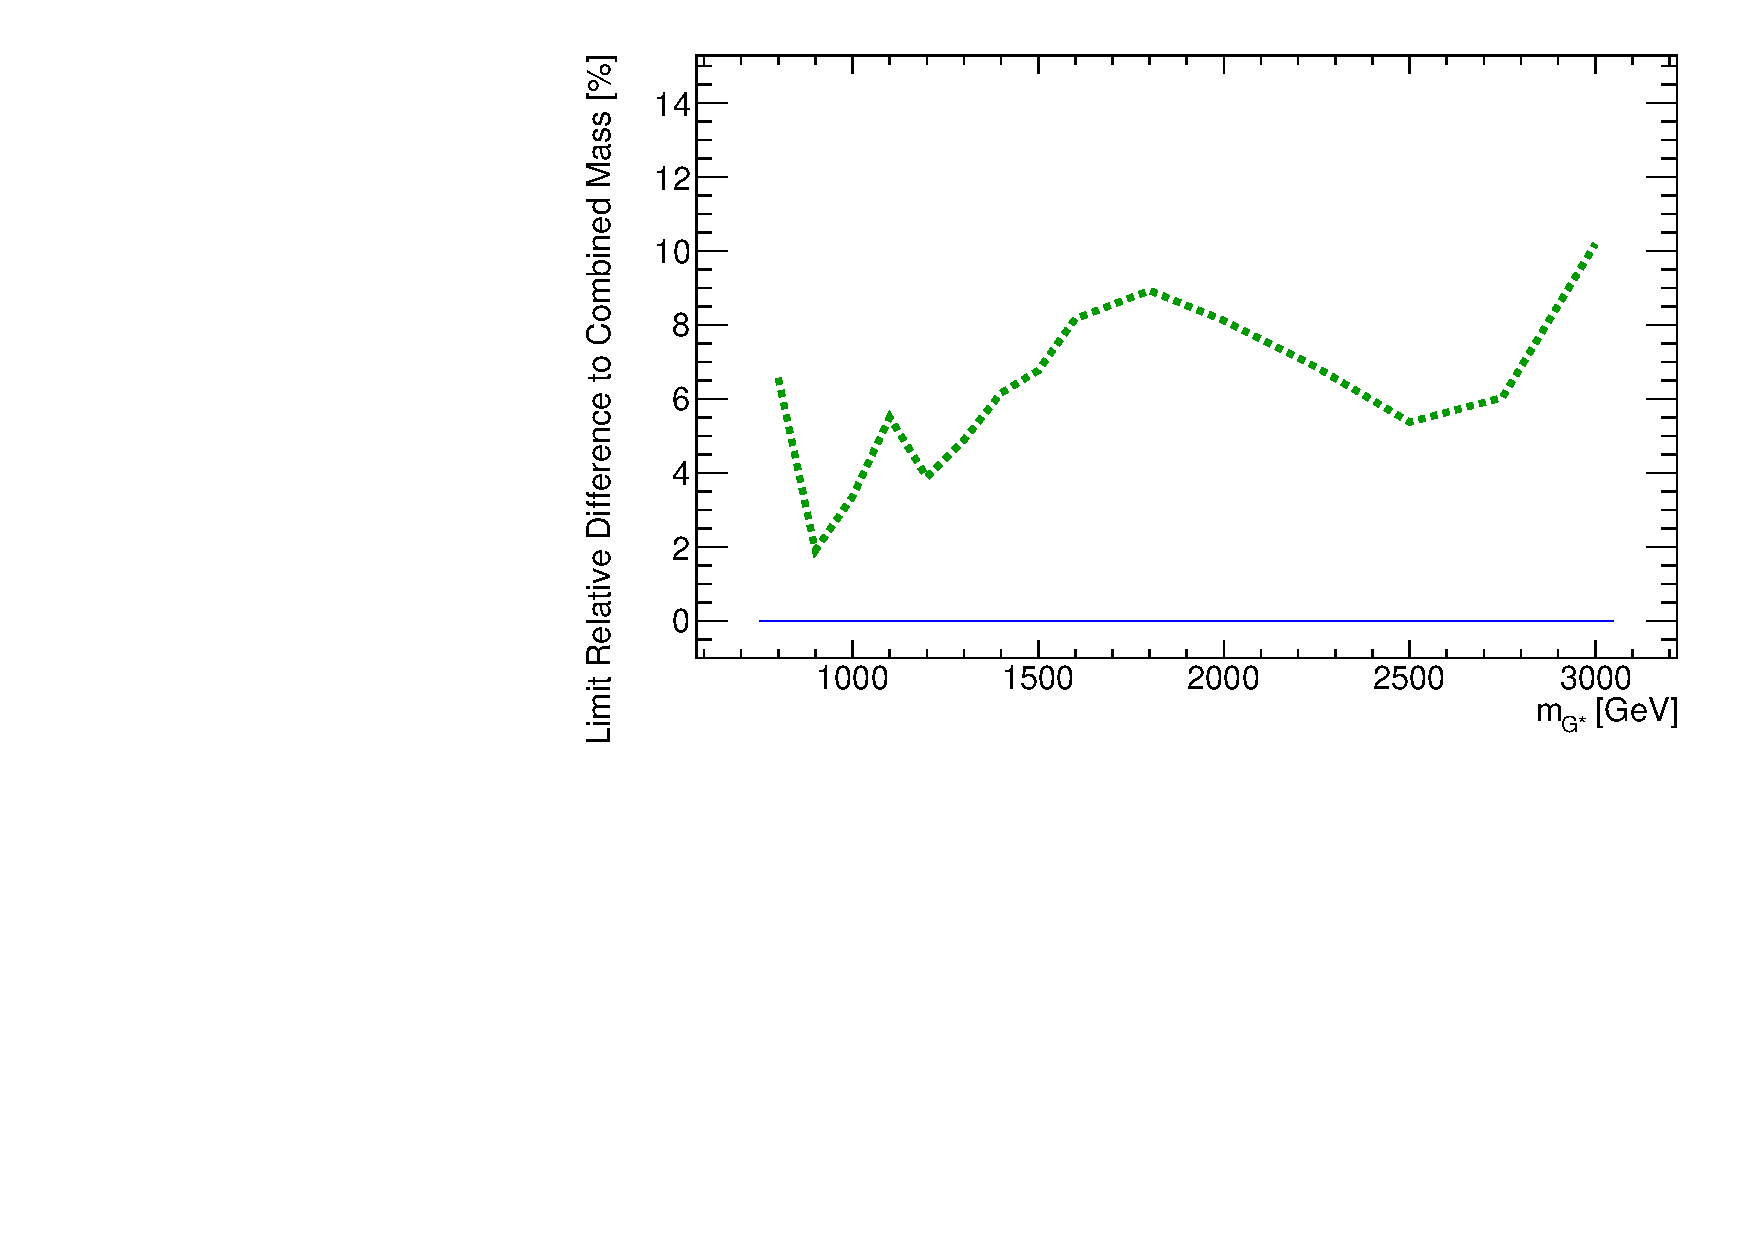
\includegraphics[angle=270, width=0.68\textwidth]{./figures/boosted/AppendixOptimization/CompareLimits_HH_BoostedNewRun2-mass_c10_ratio.pdf}
  \caption{Expected limit for combined boosted channels. The top plot is the limit for RSC $c=1.0$, and the bottom plot is the ratio of the limit relative to the blue combined mass limit. Comparison shown here are analysis repeated with calorimeter mass(green).}
  \label{fig:app-optimization-mass}
\end{center}
\end{figure*}


\clearpage
\subsection{$b$-tagging impact}
\label{sec:app-optimization-btagging}
\paragraph{}
$b$-tagging working point on track jets is chosen to be $70\%$ for this analysis, which used to be 77\%. Different $b$-tagging working points have been tested. The resulting plot is shown as Figure ~\ref{fig:app-optimization-btagging}. As seen, the $70\%$ $b$-tagging working point is better than/comparable to 77\% $b$-tagging working point in terms of cross section asympotic statistical limit, especially for higher mass signals. Hence it is chosen to be used by this analysis.

\subsection{Resolved Veto Impact}
\label{sec:app-optimization-resveto}
\paragraph{}
Impact from veto resolved events passing resolved signal region selection is shown also in Figure ~\ref{fig:app-optimization-btagging}. The impact comes mostly from 800 GeV to 1.5 TeV, with largest impact at 900 GeV, where the cross section asympotic statistical limit differes by a factor of 10. Since those events are in the resolved signal region and will be combined in the final statistical limit, it won't harm the overall resolve-boosted combined result.

\begin{figure*}[htbp!]
\begin{center}
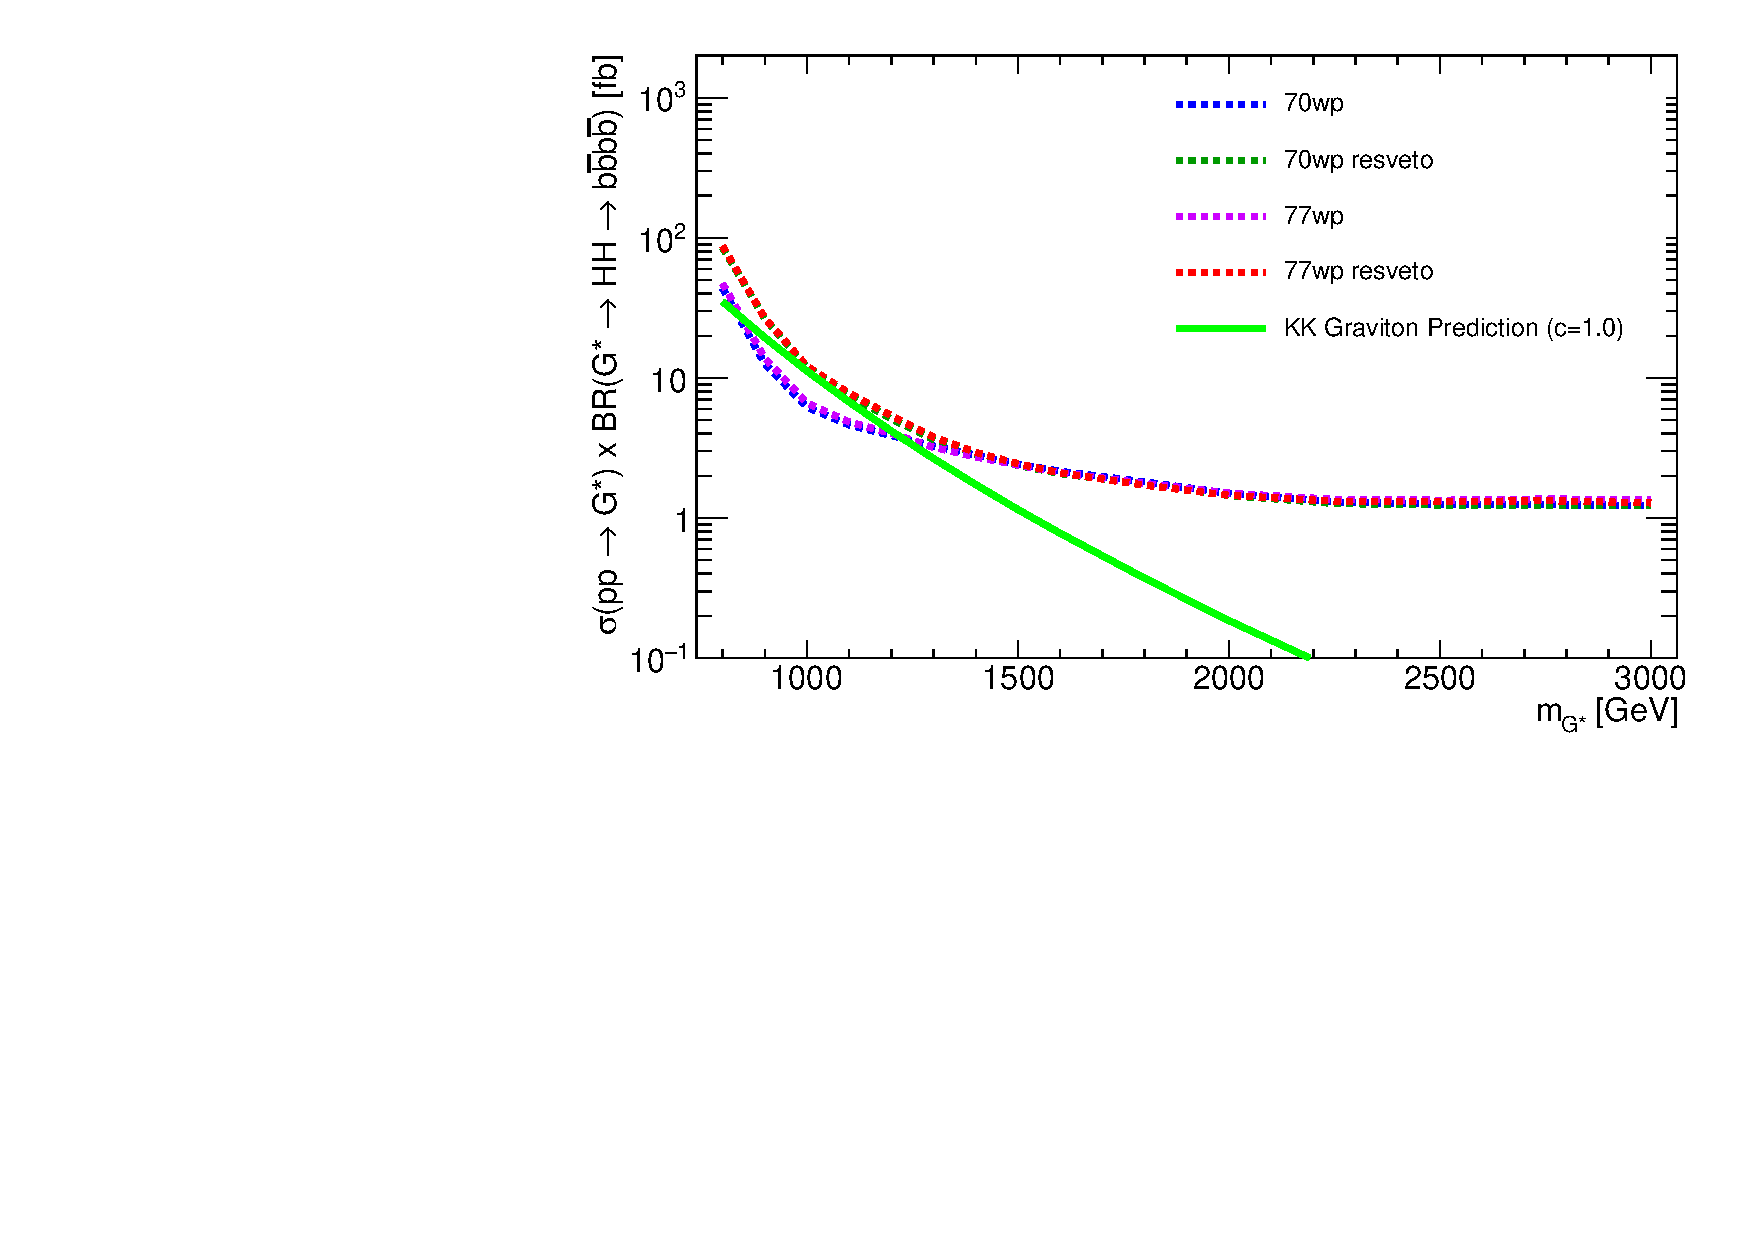
\includegraphics[angle=270, width=0.6\textwidth]{./figures/boosted/AppendixOptimization/CompareLimits_HH_BoostedNewRun2-resveto_c10.pdf}\\
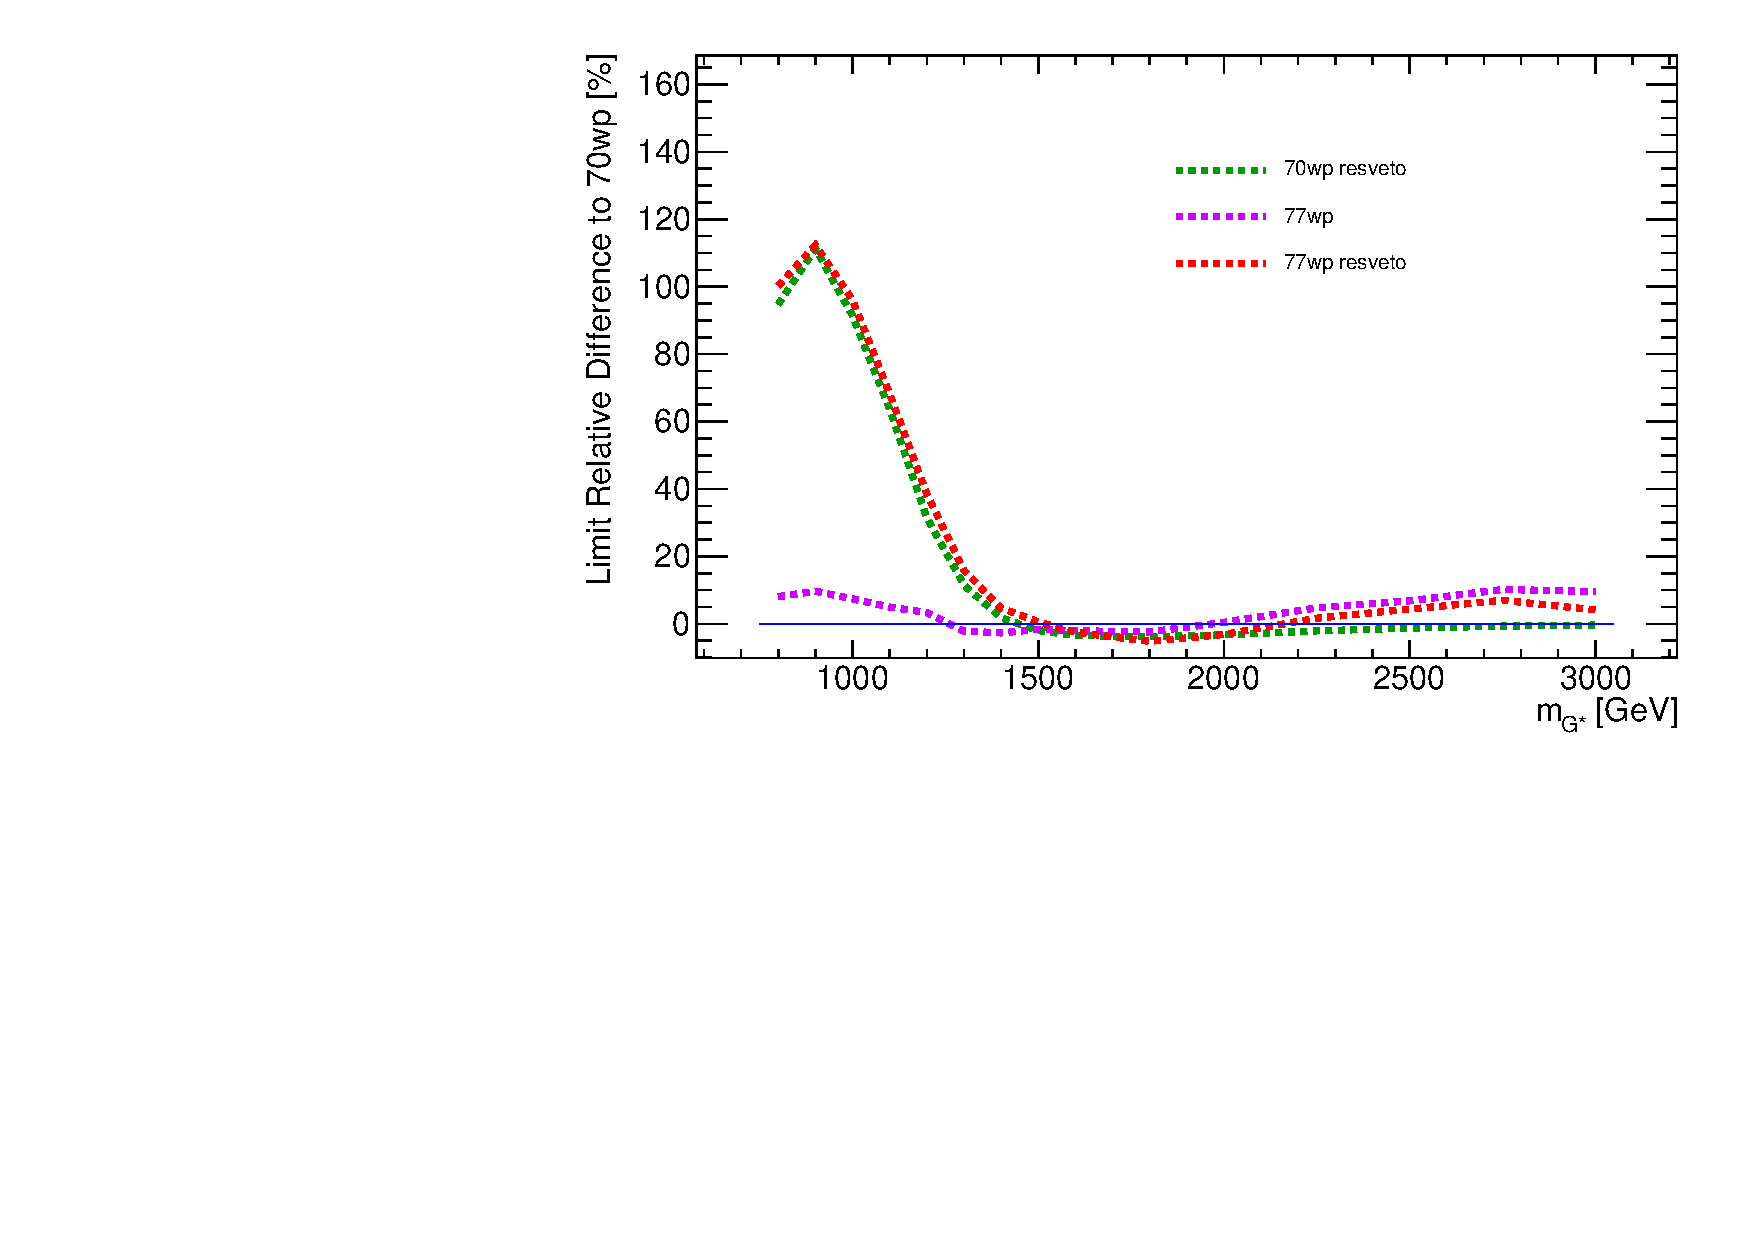
\includegraphics[angle=270, width=0.6\textwidth]{./figures/boosted/AppendixOptimization/CompareLimits_HH_BoostedNewRun2-resveto_c10_ratio.pdf}
  \caption{Expected limit for combined boosted channels. The top plot is the limit for RSC $c=1.0$, and the bottom plot is the ratio of the limit relative to the blue 70\% $b$-tagging working point limit. Comparison shown here are analysis repeated with 70\% working point but with resovled veto (green), 77 \% working point (purple), 77\% with resolved veto (red).}
  \label{fig:app-optimization-btagging}
\end{center}
\end{figure*}


\clearpage
\subsection{Scaled Mass Impact}
\label{sec:app-optimization-polemass}
\paragraph{}
Using scaled mass helps to be consistent with the resolved analysis, and gives very similar exclusion limit as using the unscaled MJJ. The difference on the limit is minimal, as shown in Figure ~\ref{fig:app-optimization-polemass}.

\begin{figure*}[htbp!]
\begin{center}
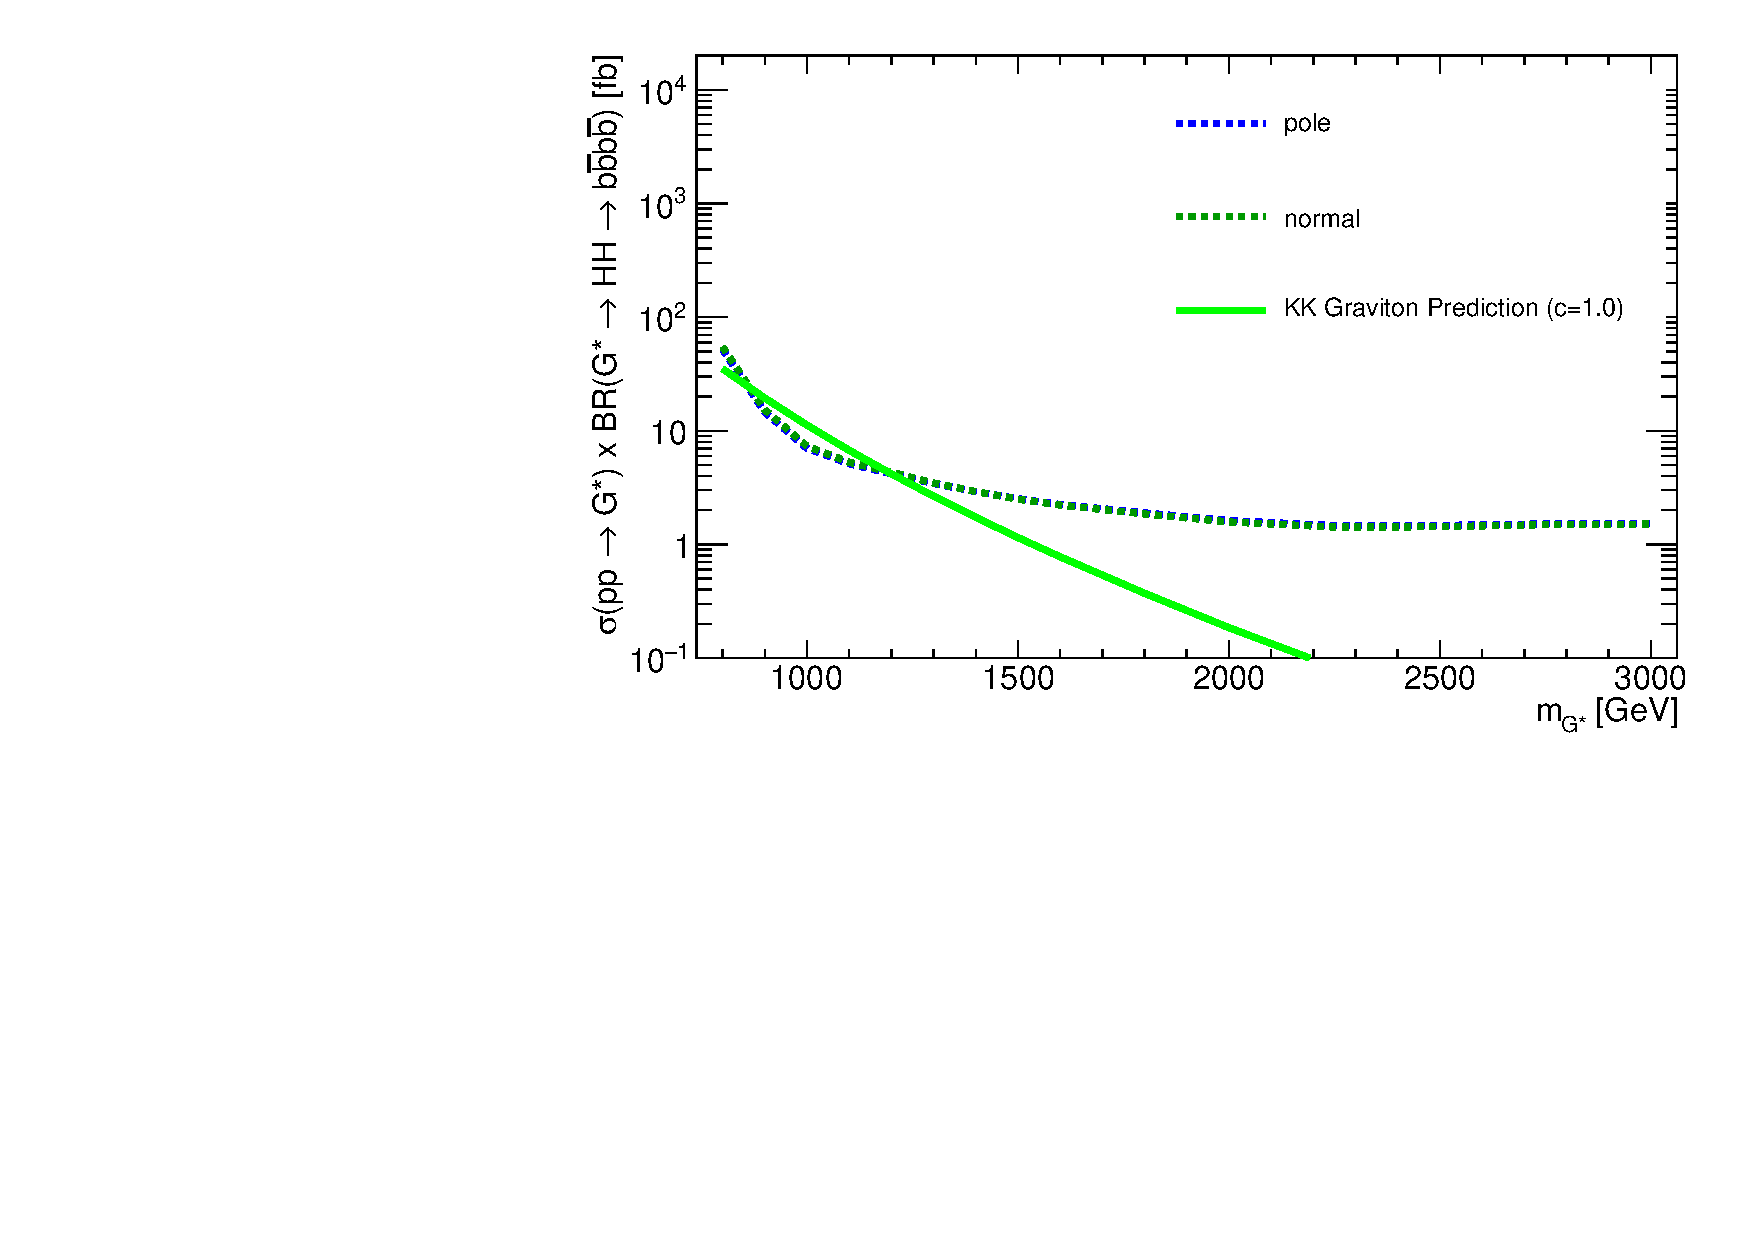
\includegraphics[angle=270, width=0.68\textwidth]{./figures/boosted/AppendixOptimization/CompareLimits_HH_BoostedNewRun2-pole_c10.pdf}\\
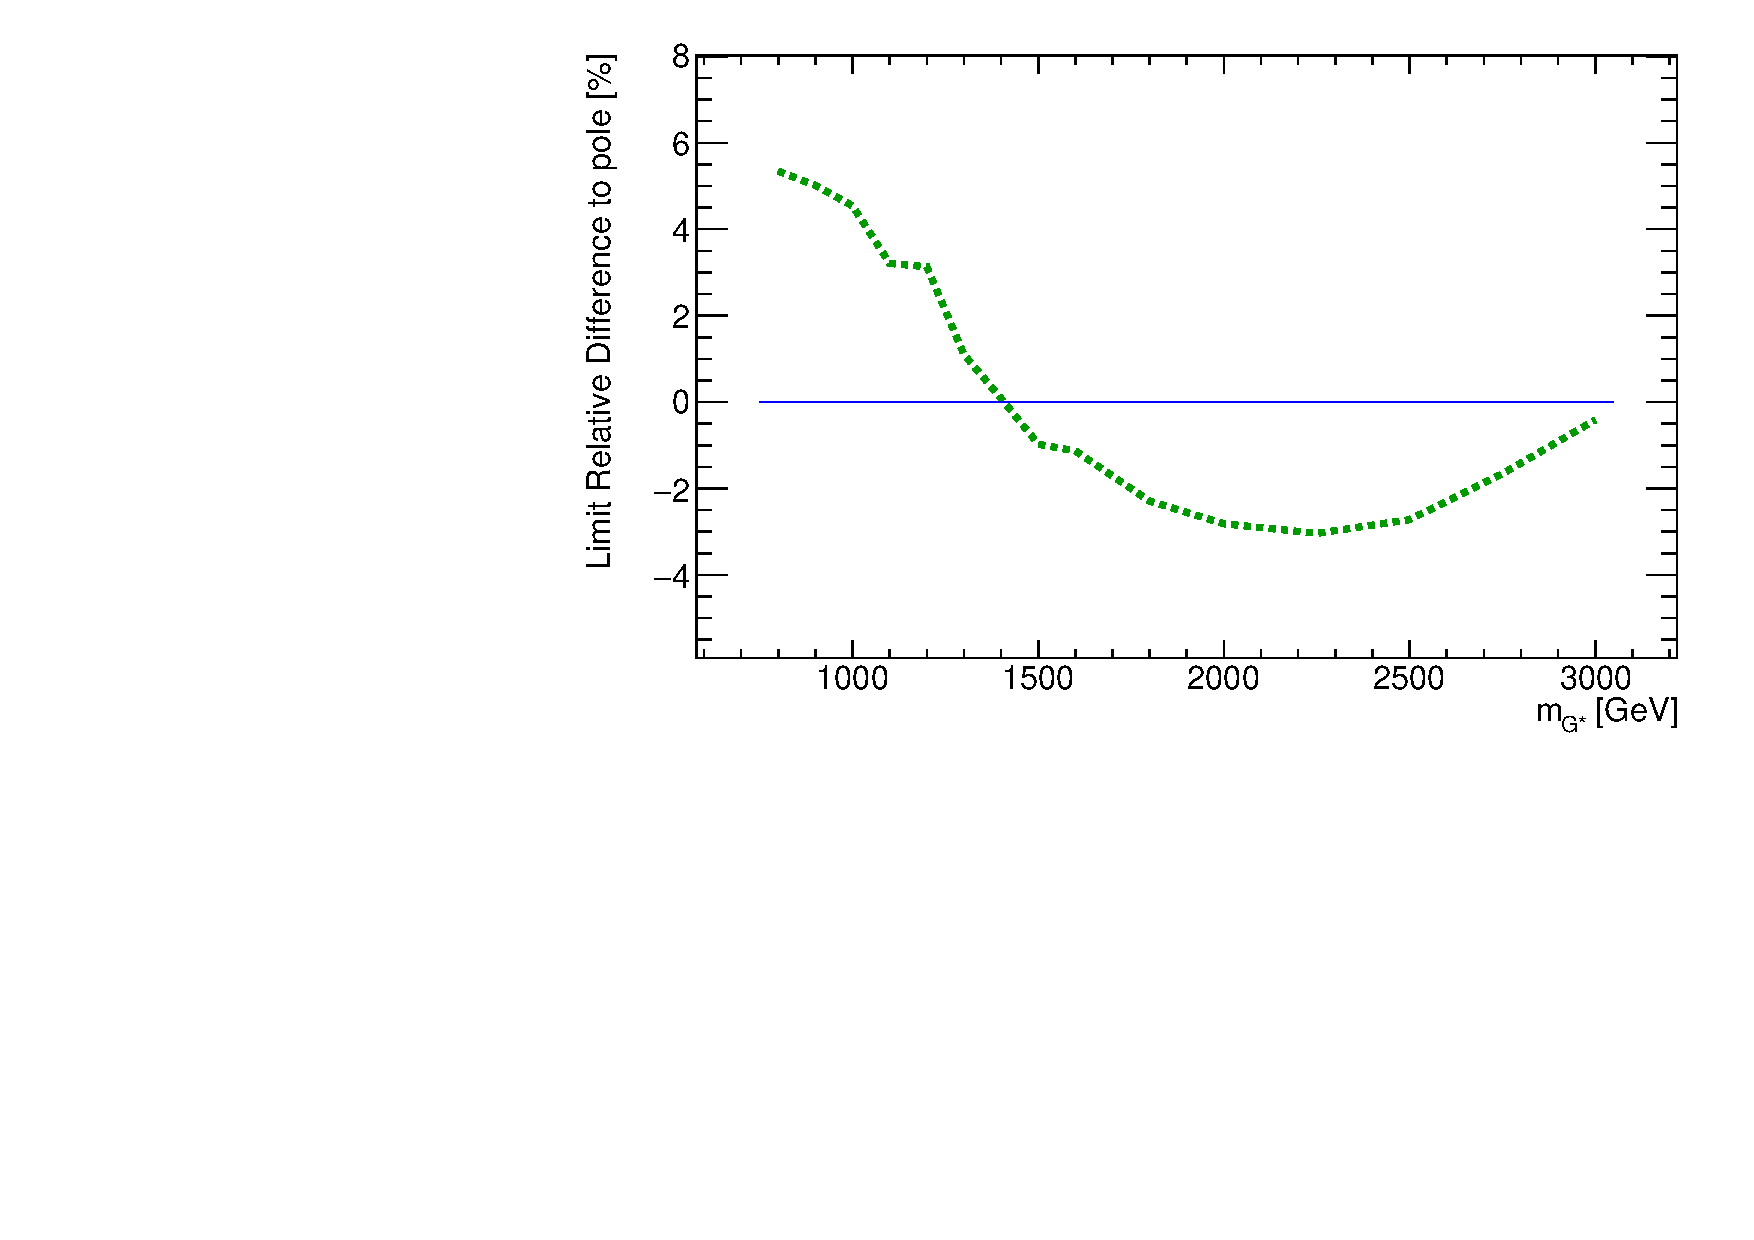
\includegraphics[angle=270, width=0.68\textwidth]{./figures/boosted/AppendixOptimization/CompareLimits_HH_BoostedNewRun2-pole_c10_ratio.pdf}
  \caption{Expected limit for combined boosted channels. The top plot is the limit for RSC $c=1.0$, and the bottom plot is the ratio of the limit relative to scaled MJJ limit. Comparison shown here are analysis repeated with unscaled MJJ (green).}
  \label{fig:app-optimization-polemass}
\end{center}
\end{figure*}

\clearpage
\subsection{Variable Radius Trackjet Impact}
\label{sec:app-optimization-vrjet}
\paragraph{}
Using variable radius (VR) trackjet's impact on the analysis is evaluated. At the time of the test, the $b$-tagging calibration on MCs is missing. The improvements mostly show for high mass signals, yet a relative lower sensitivity on the lower mass signals is found, as shown in Figure ~\ref{fig:app-optimization-vr}.

\begin{figure*}[htbp!]
\begin{center}
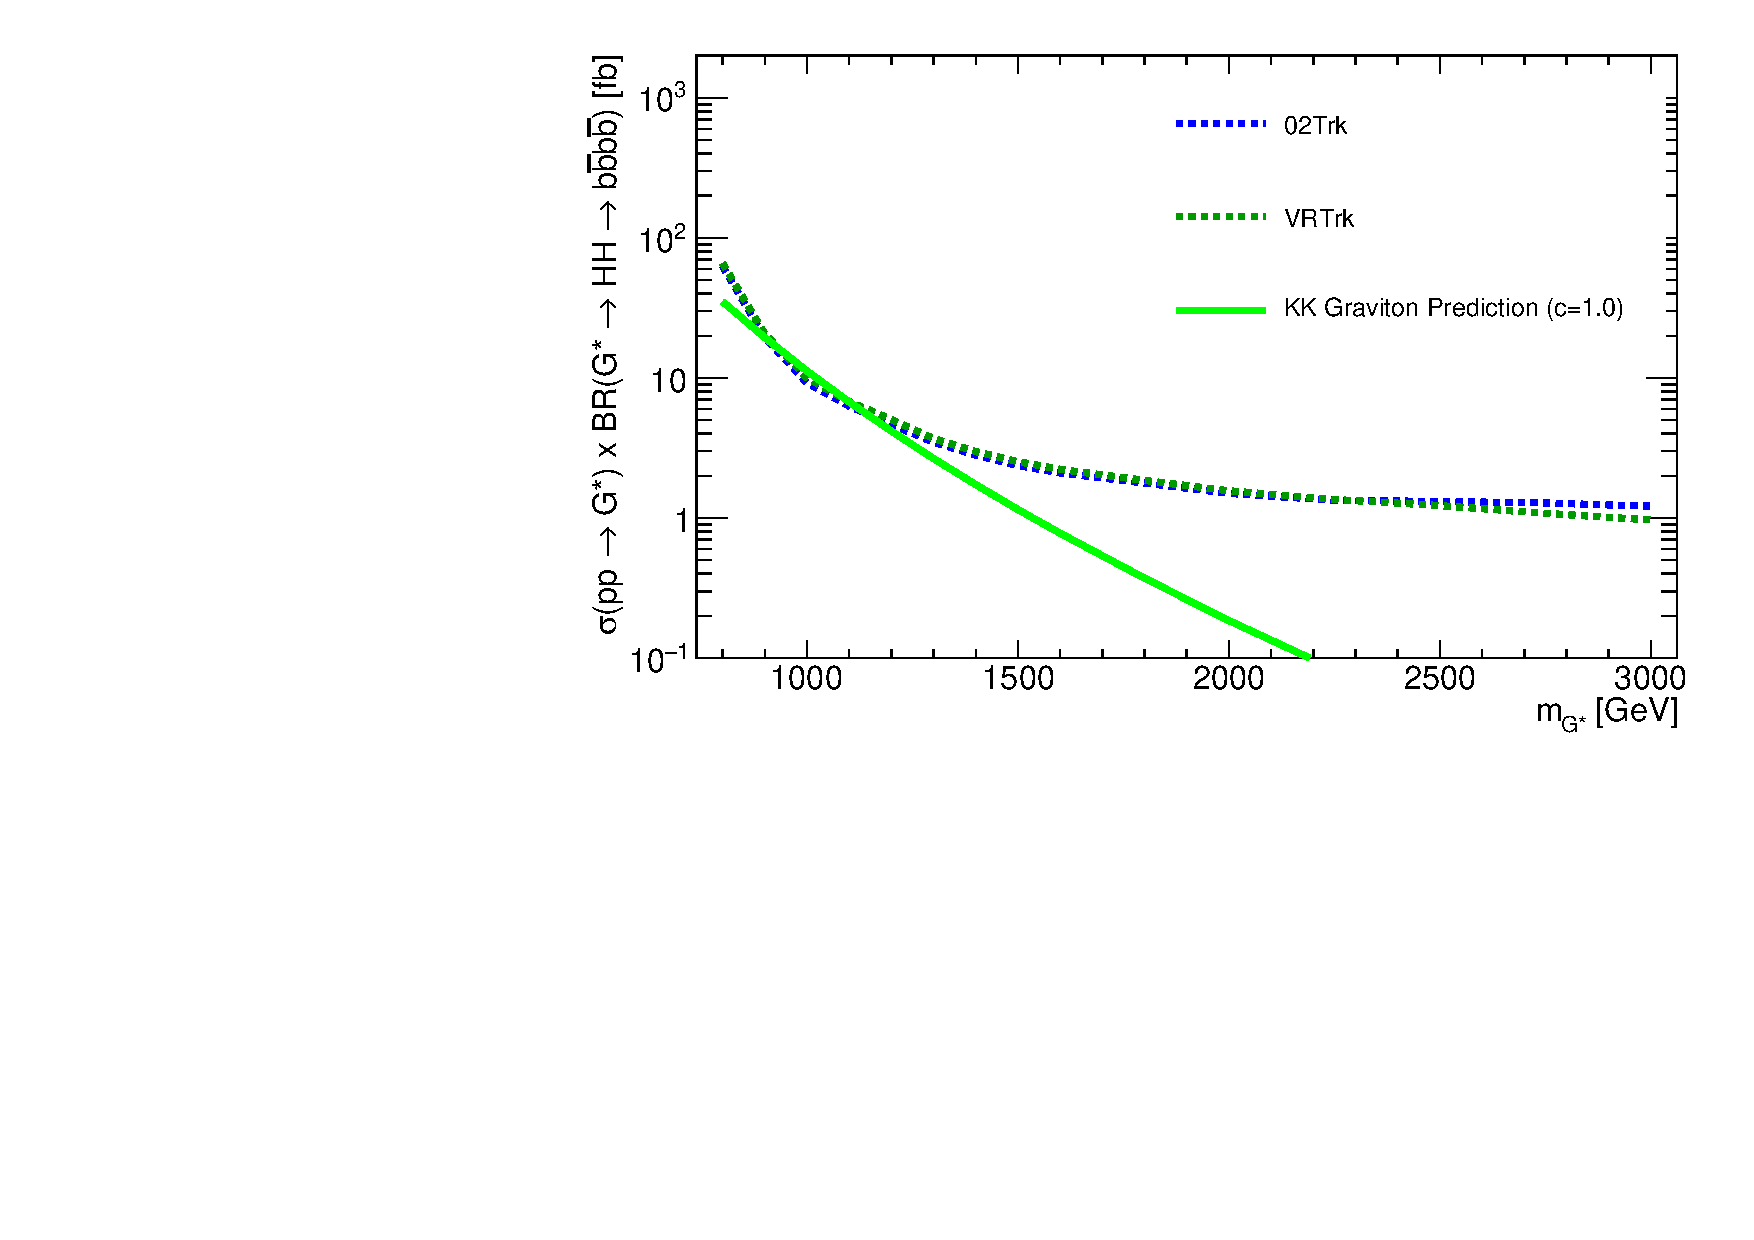
\includegraphics[angle=270, width=0.68\textwidth]{./figures/boosted/AppendixOptimization/CompareLimits_HH_BoostedNewRun2-vr_c10.pdf}\\
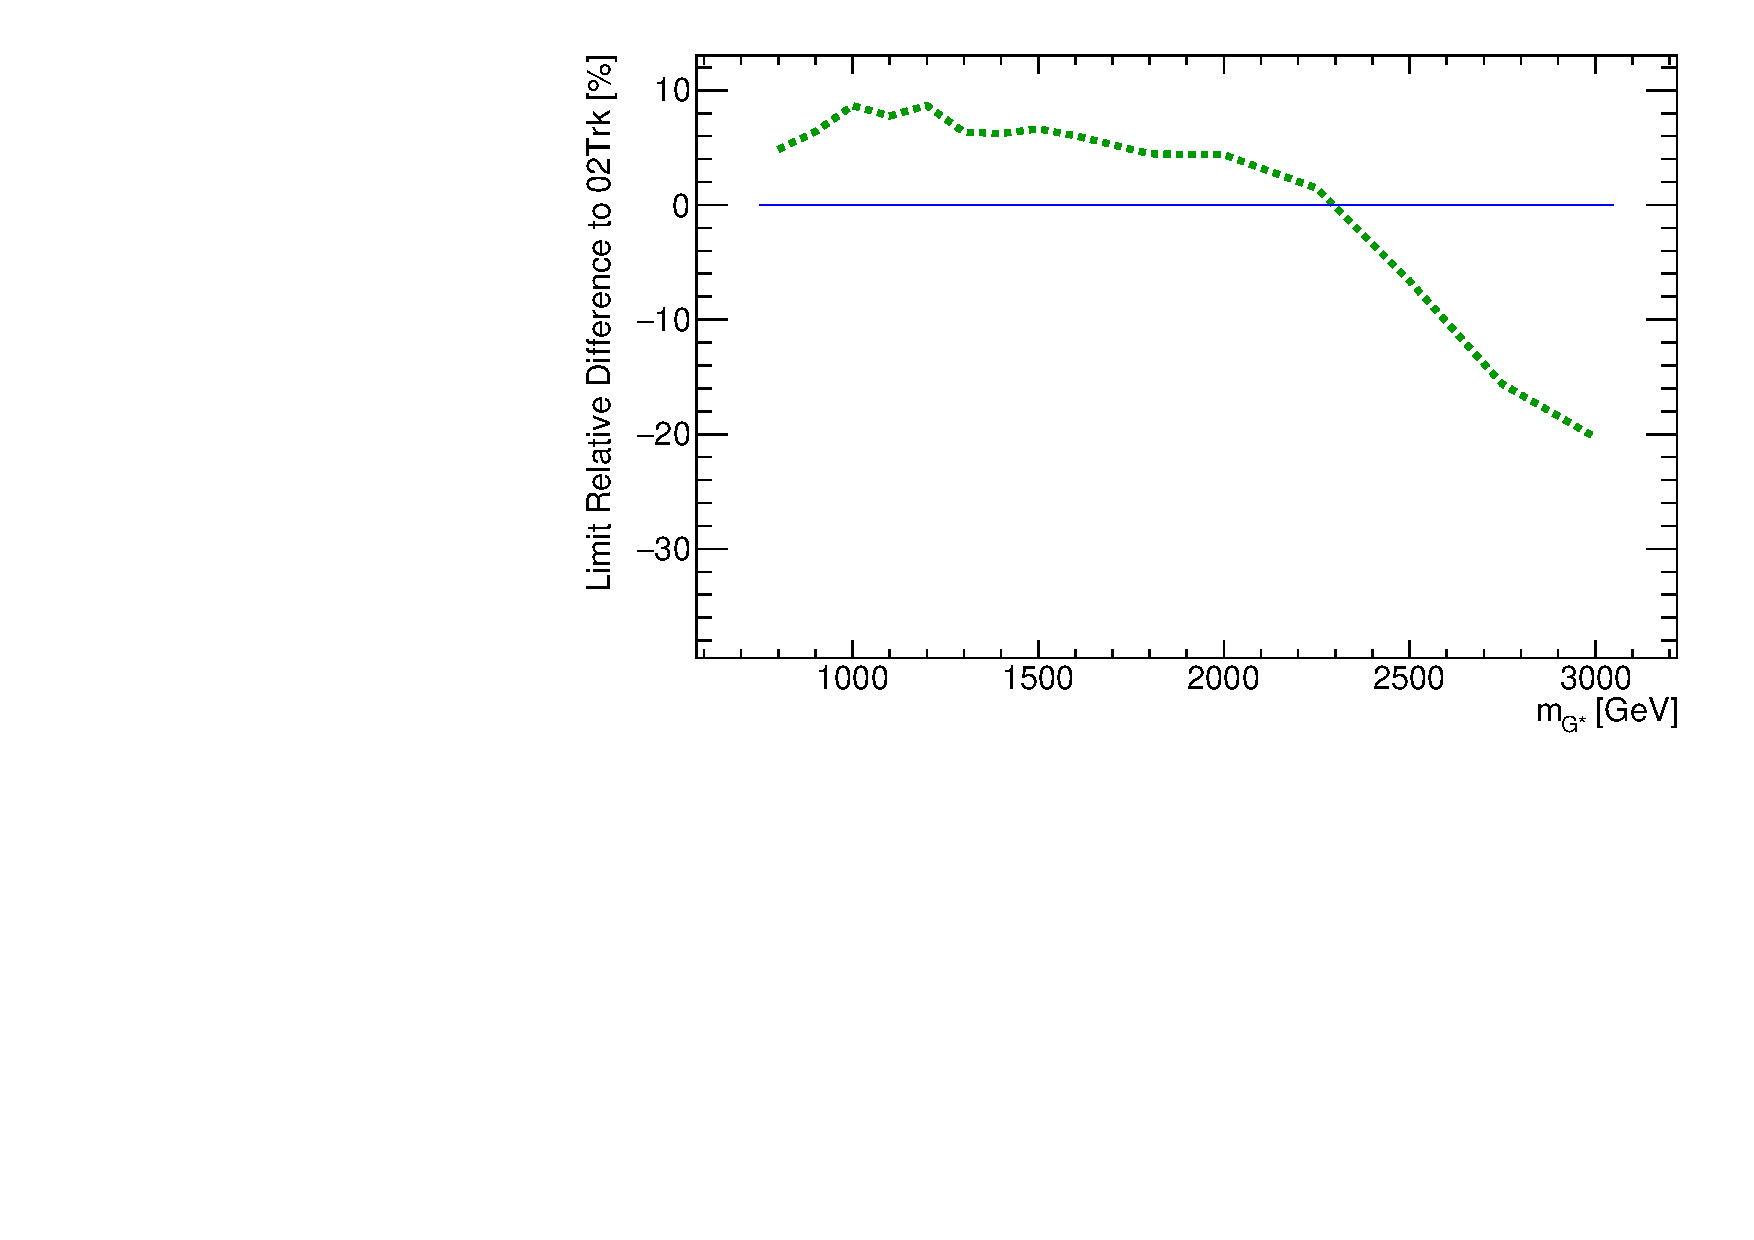
\includegraphics[angle=270, width=0.68\textwidth]{./figures/boosted/AppendixOptimization/CompareLimits_HH_BoostedNewRun2-vr_c10_ratio.pdf}
  \caption{Expected limit for combined boosted channels. The top plot is the limit for RSC $c=1.0$, and the bottom plot is the ratio of the limit relative to the standard trackjet based analysis limit. Comparison shown here are analysis repeated with variable radius track jets.}
  \label{fig:app-optimization-vr}
\end{center}
\end{figure*}

\clearpage
\subsection{Boosted Signal Region Optimization}
\label{sec:app-optimization-sr}
\paragraph{}
The signal region is optimized and the optmial expression is:
\begin{equation}
%\begin{cases}
    %\\sqrt{(\frac{m^{ lead}_{ J} - \text{124 GeV}}{0.085 (m^{ lead}_{ J})})^2 + (\frac{m^{ subl}_{ J}- \text{115 GeV}}{0.12 (m^{ subl}_{ J})})^2}, & \text{if } p_{T}^{ lead} < \text{900 GeV}\\
    %\sqrt{(\frac{m^{ lead}_{ J} - \text{124 GeV}}{0.085 (m^{ lead}_{ J})})^2 + (\frac{m^{ subl}_{ J}- \text{115 GeV}}{0.12 (m^{ subl}_{ J})})^2} - 0.4 (\frac{p_{T}^{ lead}}{\text{900 GeV}} - 1),              & \text{if} p_{T}^{ lead} \geq \text{900 GeV}
%\end{cases}
\end{equation}
which is different from the chosen signal region, as shown in Equation ~\ref{eq:boosted_XhhDef}. This optimization has two changes, the different width for leading Higgs Candidate and subleading Higgs Candidate, and the \pt dependent Xhh cut, which effectivly increase the signal region for higher resonant masses. The impact on the exclusion limit is shown in Figure ~\ref{fig:app-optimization-sr}. The improvement in exclusion limit is around 2 to 8 \%, with a strong dependence on signal mass. In order to keep the analysis simple and consitent with the resolved analysis, this signal region is not adopted.

\begin{figure*}[htbp!]
\begin{center}
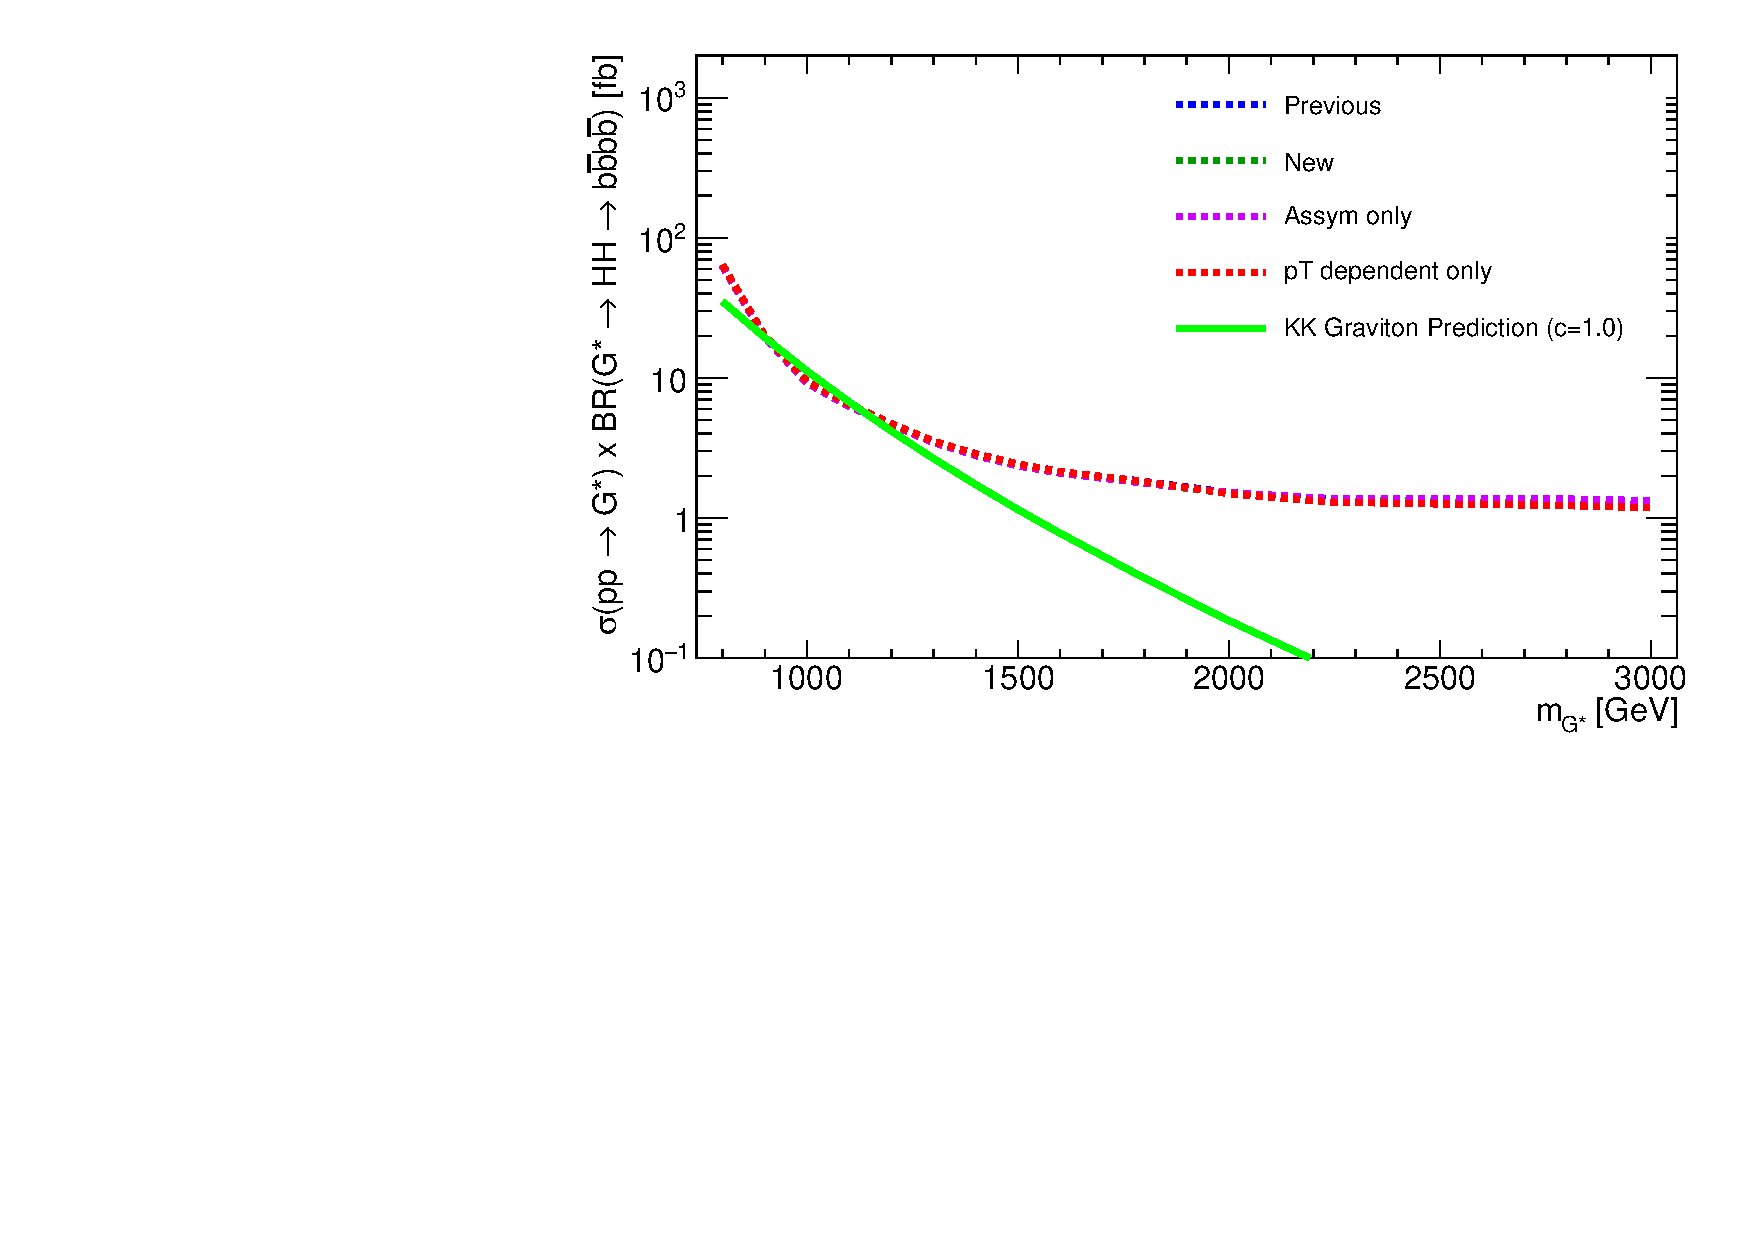
\includegraphics[angle=270, width=0.6\textwidth]{./figures/boosted/AppendixOptimization/CompareLimits_HH_BoostedNewRun2-test-SR_c10.pdf}\\
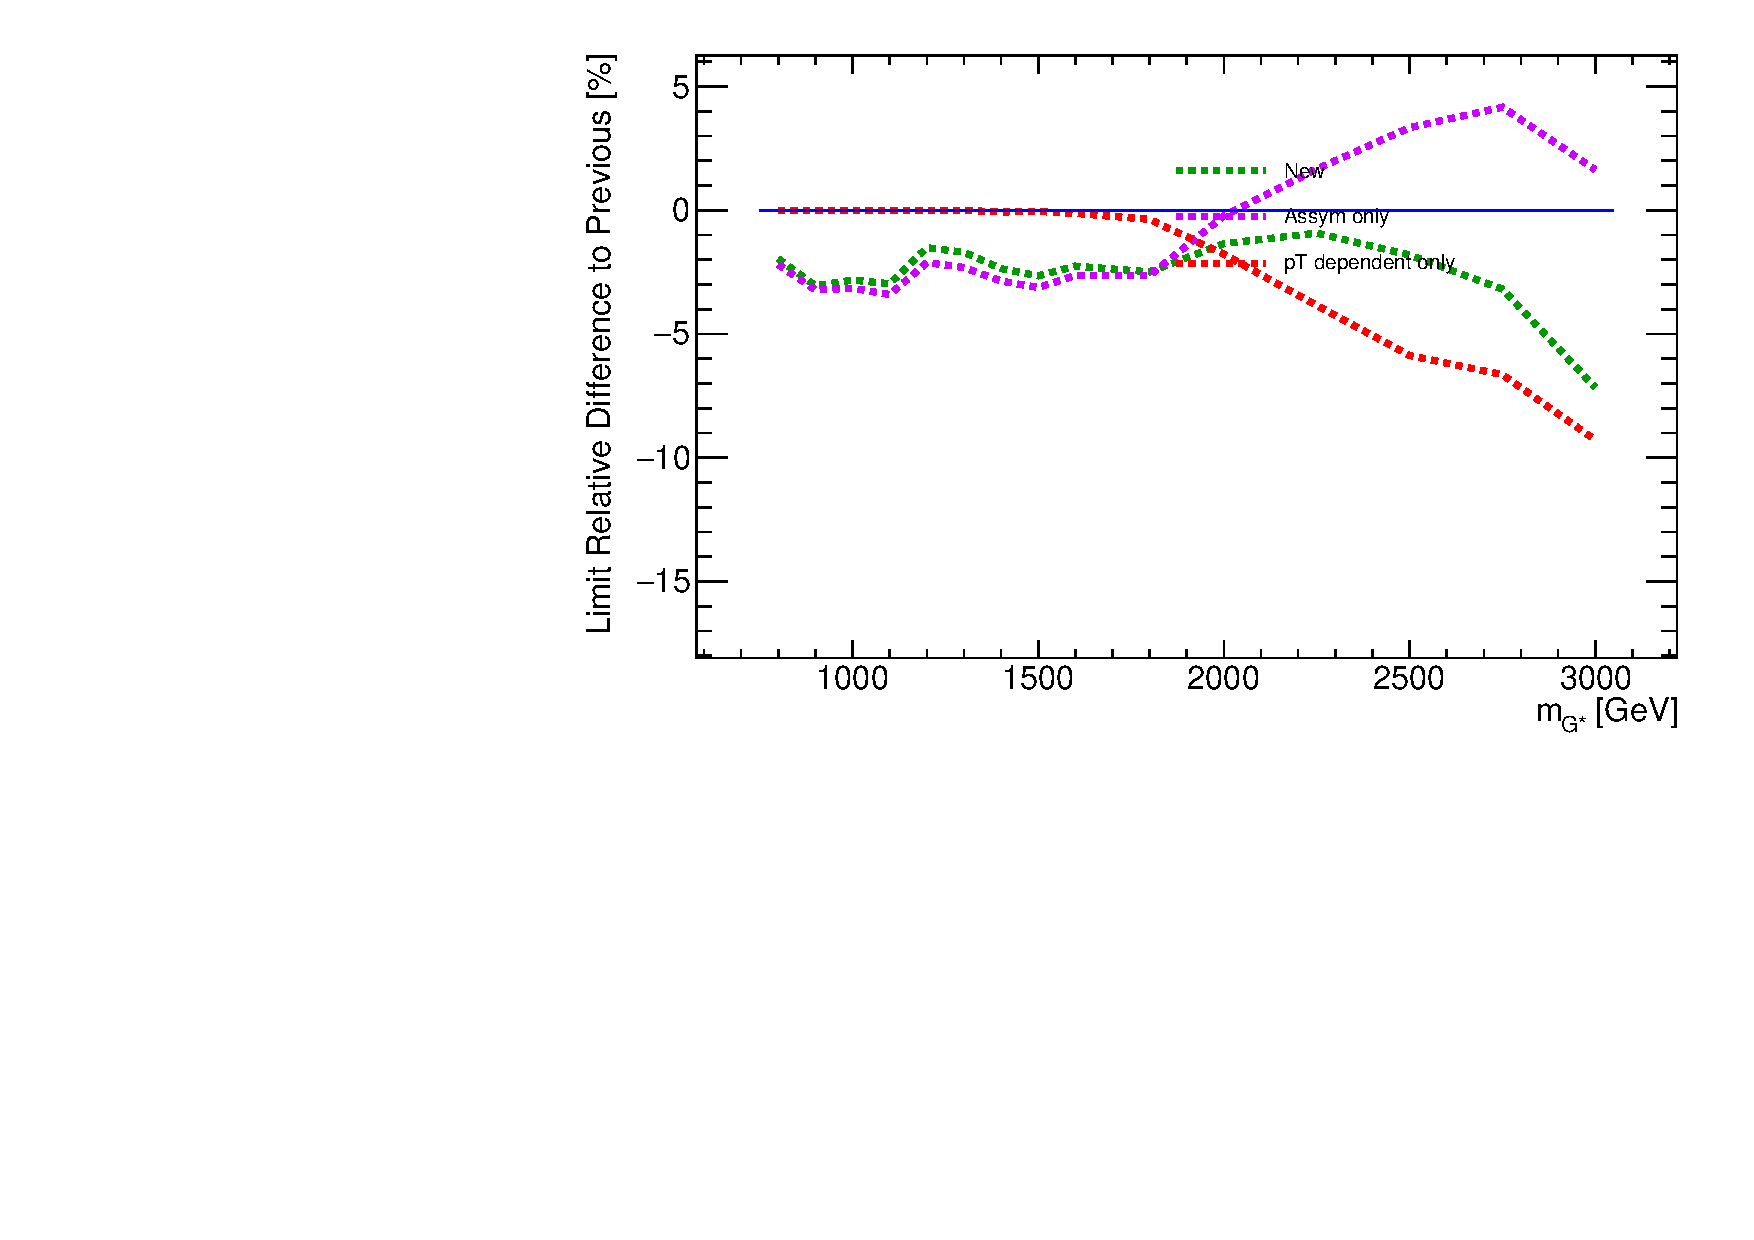
\includegraphics[angle=270, width=0.6\textwidth]{./figures/boosted/AppendixOptimization/CompareLimits_HH_BoostedNewRun2-test-SR_c10_ratio.pdf}
  \caption{Expected limit for combined boosted channels. The top plot is the limit for RSC $c=1.0$, and the bottom plot is the ratio of the limit relative to the standard signal region analysis limit. Comparison shown here are analysis repeated with the signal region defined above (new, green), with the assymetric width only (purple), and the \pt dependent Xhh cut only (red).}
  \label{fig:app-optimization-sr}
\end{center}
\end{figure*}
